\chapter{Local Automatic Differentiation}
\label{ch:LocalAD}
This chapter will consider a different approach on how to use AD to solve PDEs. When solving PDEs using a finite volume method each cell will only depend on the neighbouring cells. In the \texttt{FAD} and \texttt{CJAD} implementations, the dependencies are stored in the discrete gradient and divergence operators. The implementations calculates the residual function value and corresponding Jacobian for the whole grid simultaneously by having a vector to store the values and sparse matrices for the Jacobians. Hence when the discrete gradient and divergence operators are used in the calculation of the residual function in \autoref{ch:FlowSolver}, the Jacobian are obtained with the structure seen in \autoref{fig:flowSolverJacobian}. Local AD is a new approach that instead of calculating the residual function for all cells at once, using matrix and vector operations, it iterates through the grid and for each cell it calculates the local residual. In the end it will perform exactly the same calculations as \texttt{FAD} and \texttt{CJAD}, but instead of having large vector and matrix calculations, we now have smaller calculations concerning only one cell, and its neighbours, at the time. This new approach is based on the same idea as how AD is done in OPM \emph{\citep{OPM}}. OPM, as said in \autoref{ch:FlowSolver}, is written in C and C++ and scales better when the simulations becomes larger. It is hence interesting to see if you can write similar type of code in Julia and obtain better computational efficiency than what is achieved in MATLAB with MRST and the methods I have implemented in Julia.

\section{Implementation}
\label{sec:LADImplementation}
To get a better understanding of how local AD works, it is best to look at how it is implemented\footnote{In the following I will explain a minor simplified implementation. This is to keep the focus on the essential parts of the implementation. The left out parts will be discussed in \autoref{sec:optimizingLocalAD}}. Like for \texttt{FAD} and \texttt{CJAD} I have implemented local AD using a struct called \texttt{LAD}:
\lstinputlisting{code/LAD_structSimple.jl}
Since we now only operate on one cell at the time the implementation of local AD is simpler than for \texttt{FAD} and \texttt{CJAD}. The value of the AD-variable is now only a scalar and the Jacobian matrices is replaced by a vector of derivatives. These are the derivatives  with respect to the primary variables in the cell. For the single phase flow solver in \autoref{ch:FlowSolver}, the derivatives vector will be of length one, as each cell only contain one primary variable (pressure). The implementation of \texttt{LAD} is however with \texttt{derivatives} as a vector. This is for the opportunity to implement more complex simulations like a two or three phase simulation where each cell can contain multiple primary variables for the amount of water, oil and/or gas present in the cell (an example of a two-phase simulator can be seen in \autoref{sec:TwoPhaseSimulation}).

To make sure that each primary variable is initialized correctly, initialization of \texttt{LAD} variables is done with the \texttt{createVariable} function. This function creates a \texttt{LAD} variable with a value and a given number of derivatives. The derivative with respect to itself is set to $1.0$ while the other derivatives are zero.
\lstinputlisting{code/createVariable.jl}
The implementation of operators for the \texttt{LAD} struct is done similar as explained in \autoref{ch:Implementation} for \texttt{FAD} and \texttt{CJAD}, but since we now, instead of having a Jacobian matrix, only have a vector of derivatives, the implementation is easier and follows the lines of the description from \autoref{sec:FADWithMultipleParameters}. 

Where the implementation of the local AD tool is easier than for \texttt{FAD} and \texttt{CJAD}, there is more work when calculating the residual functions. Since we do not use discrete gradient and divergence operators, but traverse through the grid cell by cell, we need a place to store the resulting residual values and the corresponding Jacobian. We also need a method to traverse through all the cells and to calculate the contributions from each neighbouring cell. %Where the AD part of the code in \texttt{FAD} and \texttt{CJAD} were fully separated from the simulation, for local AD it is more integrated. This means that when using local AD to create the simulation it becomes a more application specific implementation than the method for \texttt{FAD} and \texttt{CJAD}. 
To create the flow solver from \autoref{ch:FlowSolver} I have chosen to store the calculated values of the residual functions in another struct called \texttt{FlowSystem}:
\lstinputlisting{code/FlowSystem.jl}
This struct look very similar to the other AD structs, except from \texttt{globalJac} being one single sparse matrix instead of a vector of sparse matrices. At this point you might not understand why it is quicker to calculate the residuals cell by cell compared to everything in one go. The key reason for this lies in the \texttt{FlowSystem} struct. Since we know that the structure of the global Jacobian will stay the same, we can reuse this sparse matrix structure throughout the whole simulation. Before the simulation begins we use the grid variable \texttt{G}, that contains the information on which cells are neighbours, and build the correct structure of \texttt{globalJac} once and for all. When we now run the simulation we only change the values inside of \texttt{globalJac}, but the structure stays the same. This reuse of \texttt{globalJac} will save a lot of memory allocations and hence speed compared to \texttt{FAD} and \texttt{CJAD} which allocates new structs for each calculation. By creating a new constructor for \texttt{FlowSystem} that uses the grid variable \texttt{G}, the variables \texttt{eqVal} and \texttt{globalJac} will be allocated with the correct length and the correct structure before the simulation begins. For the grid in \autoref{ch:FlowSolver} we have 1000 cells. This implies 1000 different pressure values and in addition we have the bottom-hole pressure (\texttt{bhp}) and the total production (\texttt{qS}). Hence \texttt{eqVal} will be a vector of length 1002.

Now that \texttt{FlowSystem} stores the  values and Jacobian of the residual functions, we need a new function to traverse through all cells and performing the calculations. The function that will execute the calculations is \texttt{assembleFlowSystem!()}, where the exclamation mark is a Julia convention for a function that modifies its input parameters. The code for \texttt{assembleFlowSystem!()} can be seen below. I have removed all declarations of help variables and replaced the code for updating \texttt{FlowSystem} with comments to highlight the important parts of the function structure.
\lstset{numbers=left}
\lstinputlisting{code/assembleFlowSystem!.jl}
\lstset{numbers=none}
The input parameter \texttt{well} is a struct that contains all necessary information about the well. The first line in \texttt{assembleFlowSystem!()} resets \texttt{eqVal} and \texttt{GlobalJac} such that the structures are unchanged, but all the values are set to zero. Then the function begin traversing through the grid and for every cell it add up the contributions from all neighbouring cells. Be aware that the looping variable names \texttt{fromCell} and \texttt{toCell} can be a bit misleading when they represent bottom-hole-pressure and total production, as those primary variables do not belong to any cell. The intuitiveness of considering the flow from one cell to another is however considered more valuable than the issue that they will also represent bottom-hole-pressure and total production. The \texttt{eqVal} and \texttt{globalJac} variables are updated in line number 6, 8 and 10 inside the inner loop. As a reminder, the residual functions that \texttt{FlowSystem} eventually will represent are the functions \texttt{presEq}, \texttt{rateEq} and \texttt{ctrlEq} defined in \autoref{sec:setupGovEq}:
\lstinputlisting{code/governingEquationsPresSolver.jl}
In line number 6, \texttt{fromCell} and \texttt{toCell} are equal, but not the bottom-hole-pressure or total production. Here the first term in \texttt{presEq}, or the backward Euler term, is calculated. This is performed in an outer function called \texttt{timeDerivative()} that returns a \texttt{LAD} struct:
\lstinputlisting{code/timeDerivative.jl}
In \texttt{FAD} and \texttt{CJAD} we made all the primary AD-variables before the simulation. We then used them as input parameters in the residual functions that returned new AD-variables which represented the values and Jacobians. With local AD we create new primary AD-variables for the applicable cell inside the function we want to evaluate. For \texttt{timeDerivative()} we create a \texttt{LAD} primary variable that represent the pressure in the cell before we calculate the backward Euler term. When \texttt{timeDerivative()} have returned the new \texttt{LAD} variable, \texttt{assembleFlowSystem!()} adds the calculated value to the correct index in \texttt{eqVal} and the derivative value to the correct diagonal index in \texttt{globalJac}.

In line number 10, when \texttt{fromCell} and \texttt{toCell} are two neighbouring cells, the divergence term in \texttt{presEq} is calculated. Like for \texttt{timeDerivative()}, we create the primary AD-variables inside the function, but since we calculate the flux from one cell to another we have to be careful with which direction we calculate the flux and which cell we want the derivative with respect to. Since the varying variables is named \texttt{fromCell} and \texttt{toCell} it is natural that the function \texttt{flux()}, seen below, calculates the flux from \texttt{fromCell} to \texttt{toCell}. 
\lstinputlisting{code/fluxFunctionLocalAD.jl}
What needs to be chosen is which cell we want the derivative with respect to. The choice only affect which indices of the Jacobian the calculated derivatives should be added or subtracted to. In \texttt{flux()} I have decided to calculate the derivative with respect to \texttt{fromCell}. The two first lines shows the consequence of this where \texttt{pFrom} is initialized with a derivative of $1$ and \texttt{pTo} as a constant. This choice leads to the following code for updating \texttt{FlowSystem} at line number 10 in \texttt{assembleFlowSystem!()}:
\lstinputlisting{code/fluxCodeLocalAD.jl}
The value of \texttt{fluxLAD} is added to \texttt{eqVal} and the derivative of the flux with respect to \texttt{fromCell} is added to \texttt{globalJac}. In addition we know that the flux from \texttt{fromCell} to \texttt{toCell} is the same as from \texttt{toCell} to \texttt{fromCell}, but with negative sign. This means that the derivative of the flux from \texttt{toCell} with respect to \texttt{fromCell} needs to be subtracted with \texttt{fluxLad.derivatives}. For a facet between two neighbours we will with \texttt{assembleFlowSystem!()} calculate the value of the flux through the facet twice, only with different signs. You might think that we could save time by subtracting \texttt{fs.eqVal[toCell]} with \texttt{fluxLAD.val}, but since we also will need the opposite derivatives of this particular flux, there will small, or next to none, computational gain of exploiting this fact. In worst case it might actually become a slower implementation, as we will have to keep track of which fluxes has been added to which cells. When the flux from all the neighbours has been added up for a cell, we have obtained the divergence in that cell. 

Line number 8 in \texttt{assembleFlowSystem!()} is the last line I have not commented and it is where the well equations, \texttt{rateEq} and \texttt{ctrlEq}, are handled. This is line is executed if both \texttt{fromCell} and \texttt{toCell} is either one of the cells containing a well, the bottom-hole pressure or the total production. The information on which cells fulfilling this condition lies in \texttt{well}. The calculation is performed by handling every case such that the correct residual functions, namely the \texttt{rateEq} or the \texttt{ctrlEq}, is calculated and added to the correct indices in \texttt{FlowSystem}.

Summed up the calculation of the residual functions using local AD is based on two modules. The first is the actual AD tool with the \texttt{LAD} struct, and the second is \texttt{FlowSystem} which keeps track of the global system and what calculations should be performed by the AD tool. With this approach we lose some of the advantages using the other AD tools where the discrete residual functions looked very similar to the continuous case, like explained in \autoref{sec:setupGovEq}. The main structure of \texttt{assembleFlowSystem!()} will however be the same no matter what type of simulation, hence making modifications to the code, or building another simulation, will not demand a complete change of the code structure. \todo{sjekk om dette ikke ble litt vagt litt senere.}

\section{Optimizing Local AD}
\label{sec:optimizingLocalAD}
As explained in the beginning of this chapter, the main idea behind local AD is to reuse the Jacobian to save memory usage and extra memory allocations. The implementation given in \autoref{sec:LADImplementation} has however left out some small, but key parts of the implementation that will massively decrease the memory and speed usage. This is purely implementation specific differences that has been left out to make the introduction to local AD more clear. It will not change the theory behind using local AD to solve PDE's.

\subsection{Dynamic VS Static Arrays}
The difference between a dynamic array and a static array is that a dynamic array can be extended or shortened as much as you like while a static array has a fixed length. Using a static array will give computational gain concerning speed and memory allocations compared to a dynamic array. This is because the compiler knows that a static array has the given fixed length forever and hence it can allocate the exact memory needed in advance and hence optimize the machine code. With a dynamic array it does not know if the array will grow larger, or smaller and it is much harder to optimize the machine code. 

Julia has a package called \emph{\cite{StaticArrays}} that provides static arrays to the the built in arrays without the possibility for changing the size of the array. The package provides two types of vectors, \texttt{SVector} and \texttt{MVector}(for two-dimensional arrays it has the corresponding \texttt{SMatrix} and \texttt{MMatrix}). Both are static vectors, but \texttt{MVector} is mutable, meaning the values inside the vector can be changed, where the values inside an \texttt{SVector} is final when the vector is defined. This makes \texttt{SVector} ideal for \texttt{LAD.derivatives} since when we perform operations on \texttt{LAD} variables, new \texttt{LAD} variables are returned.\footnote{For a multi-phase simulation, a possible implementation can be each element in the global Jacobian being an \texttt{n}$\times$\texttt{n} matrix where \texttt{n} is the number of primary variables in each cell. For this particular case an \texttt{MMatrix} is optimal to use as we know the size of the matrices, but we want to change the values inside the matrix.} 

When the implementation is changed to use static vectors it needs to know how long these vectors are. When building a simulation it is not a problem to say in advance how many derivatives we need and when the compiler knows this before compilation it can optimize the machine code. OPM solves this by creating a template class containing the length of the gradient vector.\todo{Legg til både kilde og sjekk formulering} This ensures that the compiler always knows that for this simulation, the static vector will always have this fixed length. This is important because we do not want to create \texttt{LAD} structs with different lengths for \texttt{LAD.derivatives} and we want all vectors in \texttt{FlowSystem.globalJac} to have that same length. If we define this clearly the compiler can optimize the machine code much better than if it does not know if for example some elements in \texttt{globalJac} suddenly will be allocated with a longer static mutable array. This will also make the implementation of the operators of \texttt{LAD} easier, as we know for certain that all \texttt{LAD} variables will have \texttt{derivatives} with the same length. The best implementation I have found for this in Julia is to declare a global constant variable in the local AD module such that the new implementation of \texttt{LAD} becomes:
\lstinputlisting{code/LAD_struct.jl}
One disadvantage with this implementation is that the Local AD module needs to be modified to work with simulations with more primary variables for each cell. \todo{Må se om det finnes noen annen måte, hvis ikke bør det kanskje kommenteres at det er litt krøkkete}

\section{Flow Solver with Local AD}
\label{sec:flowSolverWithLAD}
Now that \texttt{LAD} has been implemented with static vectors it is interesting to see how the local AD method compares to \texttt{FAD} and \texttt{CJAD} in the simulation from \autoref{ch:FlowSolver}. Since OPM is a simulator meant to be much faster than MRST, it is assumed that since Julia is supposed to run as fast as C, the local AD approach will give a computational gain. With the implementation given in this chapter this is however not the case. It performs worse than \texttt{CJAD} and similar to \texttt{FAD}. As explained in \autoref{sec:profiling}, profiling is an efficient way of finding the bottlenecks in a code, and this is a perfect example of when to use it - the code was expected to be faster, but it was not, so it is important to figure out if there is a small part of the code that is slow. \autoref{fig:profileSlowCreateVar} shows a screenshot of a profile result from running the flow solver simulation. The screenshot only contains blocks from the \texttt{flux()} function. Two blocks are marked with squares and two other blocks with brighter diagonal stripes. The blocks with squares are time spent in \texttt{createVariable()} and the brighter diagonal stripes are AD calculations in \texttt{flux()}.
\begin{figure}[H]
    \centering
    \begin{subfigure}[t]{0.75\textwidth}
        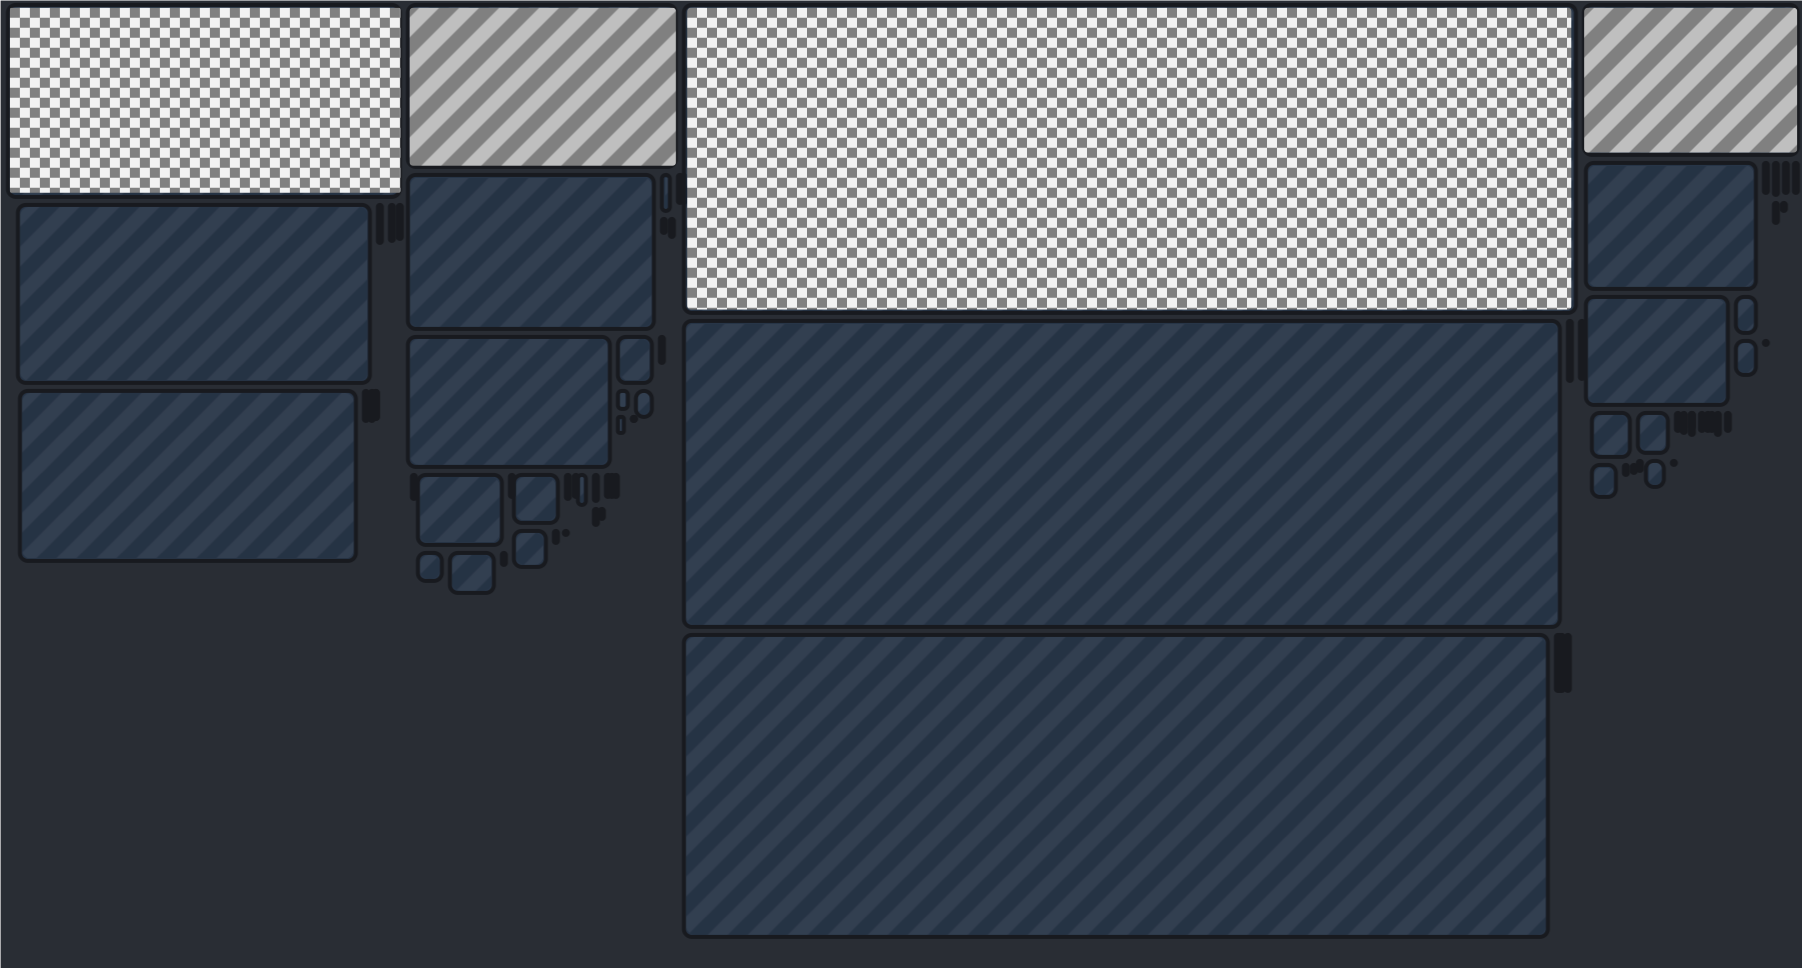
\includegraphics[height = 0.35\textheight, width=\textwidth ]{figures/profilingSlowCreateVariablesFlux.png}
        \caption{}
        \label{fig:profileSlowCreateVar}
    \end{subfigure}
    \hspace{0.06\textwidth}
    \begin{subfigure}[t]{0.18\textwidth}
        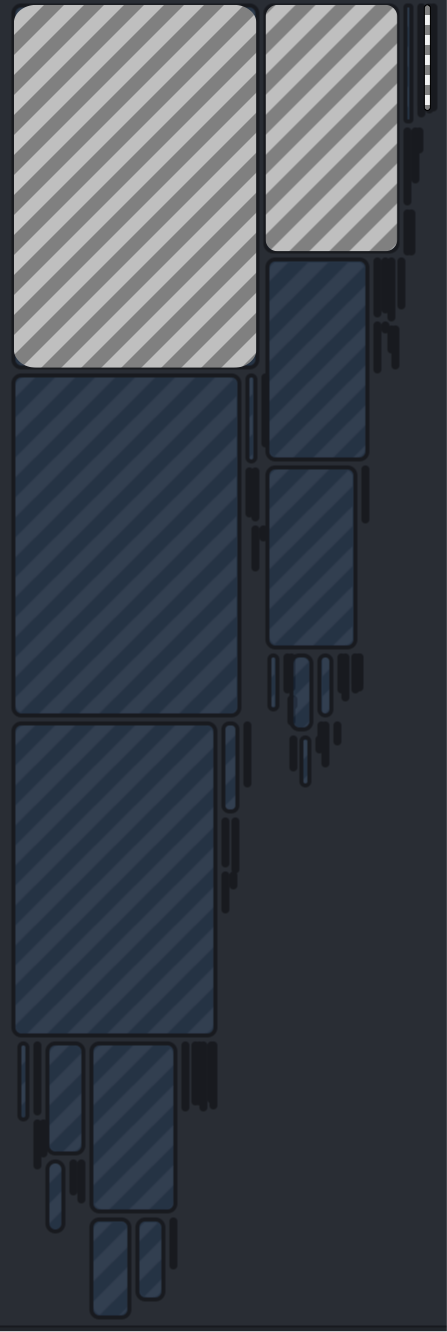
\includegraphics[height = 0.35\textheight, width=\textwidth]{figures/profilingFastCreateVariablesFlux.png}
        \caption{}
        \label{fig:profileFastCreateVar}
    \end{subfigure}
    \caption{The figures shows screenshots of the profile result from \texttt{flux()} in the flow solver simulation from \autoref{ch:FlowSolver}. The blocks marked with squares are time spent in \texttt{createVariable()} and the blocks with bright diagonal lines are calculations in \texttt{flux()}. \autoref{fig:profileSlowCreateVar} uses a slow version of \texttt{createVariable()} while \autoref{fig:profileFastCreateVar} uses a faster version.}
\end{figure}
It is suprising that creating a \texttt{LAD} struct should take more time than the actual AD calculations. This indicates that the \texttt{createVariable()} function is poorly implemented. If we look closer at the implementation we see that we only want to create a static \texttt{Svector}, but we start by creating a dynamic vector of zeros, and then we modify the vector by changing one of the values to one. Finally in the last line we convert the dynamic vector into a static \texttt{SVector}. The new implementation seen below is a Julia specific implementation where the \texttt{SVector} is created immediately with correct values and without any use of dynamic vectors.
\lstinputlisting{code/createVariableFast.jl}
The new profiling result with the updated \texttt{createVariable()} can be seen in \autoref{fig:profileFastCreateVar}. The time spent in \texttt{createVariable()} is almost eliminated and we can see that approximately all the time spent in \texttt{flux} are used for AD calculations. This is what is expected as initialization should be far less time consuming than AD calculations. 

As discussed in \autoref{ch:FlowSolver}, by only looking at assembling of the residual functions, and not the full simulation, we eliminate the linear solver from the benchmark, and we get a better understanding of how efficient the AD tools are. \autoref{tab:FlowSolverAssemblyTestWithLAD} is the same table as \autoref{tab:FlowSolverAssemblyTest}, assembling the residual functions 100 times, but with the benchmarked time for Local AD added to the end of the table.
\begin{table}[htb]
    \centering
    \caption{Table with speed benchmarks of different AD methods assembling the "Single-Phase Compressible AD Solver" residual function 100 times for different discretizations.}
    \label{tab:FlowSolverAssemblyTestWithLAD}
    \def\arraystretch{1.5}
    \begin{tabular}{ccccc}
    \textbf{Number of cells} & \textbf{FAD} & \textbf{CJAD} & \textbf{MRST} & \textbf{Local AD}\\
        \hline
         $10\times10\times10$ & 0.9s & 0.4s & 0.6s & 0.07s \\  
         $20\times20\times20$ & 9.3s & 4.0s & 3.6s & 0.6s \\ 
         $30\times30\times30$ & 44.2s& 17.2s& 16.5s & 2.2s \\ \hline
    \end{tabular}
\end{table}
The table shows that the local AD approach is approximately six times faster than the other tested implementations which is a significant improvement. This gives us an indication that Julia can be a language where we can quickly create new simulations using \texttt{CJAD} or a similar AD tool and in the same language create more efficient simulators using a method like local AD. To confirm this however, we need to test the performance for a larger problem than a single-phase pressure solver. In \autoref{sec:TwoPhaseSimulation} I will test how local AD performs in Julia as a two-phase solver for a more realistic grid structure. This will give a better indication on how well Julia is suited for creating high performance simulators.

\section{Two Phase....}
\label{sec:TwoPhaseSimulation}

\begin{table}[htb]
    \centering
    \caption{Write caption}
    \label{tab:FlowSolverAssemblyTestWithLAD}
    \def\arraystretch{1.5}
    \begin{tabular}{ccc}
    \textbf{Local AD} & \textbf{CJAD} & \textbf{MRST}\\
        \hline
        5.89s & 31.97s & 30.15s \\  
        \hline
    \end{tabular}
\end{table}


\todo[inline]{Se på parallellisering for lokal AD?}